%----------------------------------------------------------------------------------------
%	TITLE PAGE
%----------------------------------------------------------------------------------------

\renewcommand{\titlepage}[2]{
	\thispagestyle{empty} % Suppress headers and footers on the title page

	\begin{tikzpicture}[remember picture, overlay]
		\node [inner sep=0pt] at (current page.center) {#1}; % Background image
		\node [anchor=center, inner sep=1.25cm, rectangle, fill=maincolor!20!white, fill opacity=0.3, text opacity=1, minimum height=\paperheight, minimum width=\paperwidth, text width=0.8\paperwidth] at (current page.center) {#2}; % Title highlight box with title(s) and author(s)
	\end{tikzpicture}
	
	\newpage
}
\titlepage % Output the title page
	{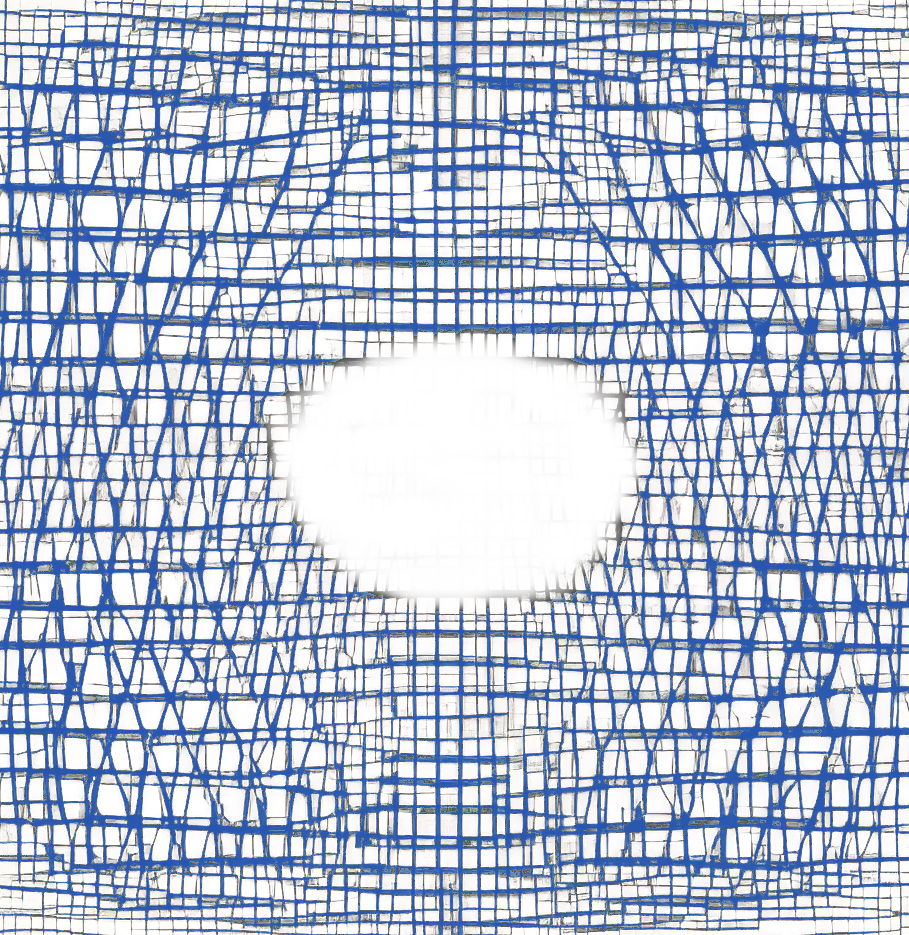
\includegraphics[width=\paperwidth,height=\paperheight]{images/cover.png}} % Code to output the background image, which should be the same dimensions as the paper to fill the page entirely; leave empty for no background image
	{ % Title(s) and author(s)

		\centering\sffamily % Font styling
		\par
		\vspace{10pt}
		\par
		{\Huge\bfseries Teoria de Galois\par} % Book title
		\vspace{16pt} % Vertical whitespace
		{\LARGE\bfseries Marc Masdeu\par} % Author
		\vspace{20pt} % Vertical whitespace
		{\LARGE\bfseries UAB\par}
	}


%\begingroup
%\thispagestyle{empty} % Suppress headers and footers on the title page
%\begin{tikzpicture}[remember picture,overlay]
%\node[inner sep=0pt] (background) at (current page.center) {};
%\draw (current page.center) node [fill=maincolor!30!white,fill opacity=0.6,text opacity=1,inner sep=1cm]{\Huge\centering\bfseries\sffamily\parbox[c][][t]{\paperwidth}{\centering Teoria de\\Galois\\[15pt] % Book title
%{\Large Marc Masdeu, UAB}\\[10pt]
%}};
%\end{tikzpicture}


% \vfill
% \endgroup

% \begin{center}
% https://tikzcd.yichuanshen.de/#N4Igdg9gJgpgziAXAbVABwnAlgFyxMJZAVgBoAGAXVJADcBDAGwFcYkQAdDgRW4AoucAI4AnHMgAsAX2AAmKaSwBKEAvSZc+QijIBGanSat2XXgI7CxchctWl12PASJlZBhizaJOPfrbUgGI5aLqQAzO5GXj68dg6azigAHKT6NB7G3qb8fLoAtMqCouISlNYqAUEJ2si65KmRnia+fLkA1IUWxZJl8nGBGk41AJykbulRzWZYRVbyFfYDwYnIsg0TTVktM11iPeX9VUNE9WmGmzH8syW9Ugvxxyi6Y42Zl+aWOAdSBjBQAObwIigABmIggAFskPUQDgIEhniAABYwehQdiQMBsAJgyHQmhwpApZGo9HeTHYxa4qGIGGExAAdhoKLRGIIlNB4JpiPpaxJrPJ7P61KQfPpYWZpLZWOFXKQo1h8MQEv5ZPAQpxcsZBKVCpZaopsrxiGJ9L1UsFMs1xrpSokkoF6qtVK1tqQZFV0o5IBFiHtiqQADYaIwsDLvHAIKH0Q6DUKCfQsIwvSAQ-QAEYwRgABUGIW8jBgIJwRppHvpwc9lu9vsr4tjKZ+UiAA
% \begin{tikzcd}[column sep=small, row sep=large]
%   &                                      &                                         &  &  & {\QQ(\sqrt[4]{2},i)} \arrow[d, no head] \arrow[llllld, no head] \arrow[llld, no head] \arrow[rrrd, no head] \arrow[rrrrrd, no head] &  &  &                                             &                                       &                                            \\
%   {\QQ(\sqrt[4]{2})} \arrow[rd, no head] &                                      & {\QQ(i\sqrt[4]{2})} \arrow[ld, no head] &  &  & {\QQ(\sqrt{2},i)} \arrow[d, no head]                                                                                                &  &  & {\QQ((1-i)\sqrt[4]{2})} \arrow[rd, no head] &                                       & {\QQ((1+i)\sqrt[4]{2})} \arrow[ld, no head] \\
%   & \QQ(\sqrt{2}) \arrow[rrrrd, no head] &                                         &  &  & \QQ(i) \arrow[d, no head]                                                                                                           &  &  &                                             & \QQ(i\sqrt{2}) \arrow[lllld, no head] &                                            \\
%   &                                      &                                         &  &  & \QQ                                                                                                                                 &  &  &                                             &                                       &                                           
% \end{tikzcd}
% \end{center}
  

%----------------------------------------------------------------------------------------
%	COPYRIGHT PAGE
%----------------------------------------------------------------------------------------

\newpage
~\vfill
\thispagestyle{empty}

\noindent Copyright \copyright\ 2023 Marc Masdeu\\ % Copyright notice

% \noindent \textsc{Published by Publisher}\\ % Publisher

% \noindent \textsc{book-website.com}\\ % URL

\noindent Aquesta obra està subjecta a una llicència de Reconeixement 3.0 No adaptada de Creative Commons


%----------------------------------------------------------------------------------------
%	TABLE OF CONTENTS
%----------------------------------------------------------------------------------------

\usechapterimagefalse % If you don't want to include a chapter image, use this to toggle images off - it can be enabled later with 

\pagestyle{empty} % Disable headers and footers for the following pages


\tableofcontents % Print the table of contents itself

\cleardoublepage % Forces the first chapter to start on an odd page so it's on the right side of the book

\pagestyle{fancy} % Enable headers and footers again
